\section{Vàlvules distribuïdores}

Una vàlvula és com un \textbf{semàfor per a l'aire}: decideix per on passa i per on no. Sense vàlvules l'aire arribaria a tot arreu alhora i no podríem controlar res.

\begin{idea}
Una \textbf{vàlvula} és un element que permet \textbf{distribuir o regular} l'aire dins del circuit. Les \textbf{vàlvules distribuïdores} obren, tanquen o desvien el pas de l'aire comprimit. Es nomenen amb \textbf{dues xifres}:
\[ \boxed{\ \text{nombre de vies}\ /\ \text{nombre de posicions}\ } \]
\begin{itemize}
 \item Les \textbf{vies} són les connexions d'aire de la vàlvula (els forats per on entra o surt l'aire).
 \item Les \textbf{posicions} són les formes diferents en què es pot connectar l'aire dins de la vàlvula.
\end{itemize}
Una vàlvula \textbf{3/2} té 3 vies i 2 posicions; una de \textbf{5/2}, 5 vies i 2 posicions.
\end{idea}

\subsection*{Com es llegeix el símbol}

\begin{itemize}
 \item Cada \textbf{quadrat} és una \textbf{posició} de la vàlvula.
 \item Les \textbf{línies que surten} dels quadrats són les \textbf{vies} (connexions amb l'exterior).
 \item A dins dels quadrats, les \textbf{fletxes} indiquen per on passa l'aire i les \textbf{T} indiquen que la via està \textbf{tapada}.
 \item Les connexions exteriors es dibuixen sempre a la \textbf{posició de repòs} (la del costat de la molla). Per saber què fa la vàlvula quan l'accionem, ens imaginem que l'altre quadrat es desplaça fins a les connexions.
 \item Les vies es numeren: \textbf{1} = alimentació (entrada d'aire a pressió), \textbf{2} i \textbf{4} = utilització (cap a l'actuador), \textbf{3} i \textbf{5} = escapament (surt a l'atmosfera, es dibuixa amb un petit triangle).
\end{itemize}

\begin{center}
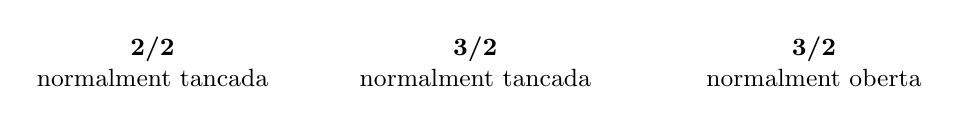
\begin{tikzpicture}[x=1cm,y=1cm]
 \pnvalve{a}{0}{0}{22nc}{man}{spring}
 \pnportnum{a}{1}{below}\pnportnum{a}{2}{above}
 \node[font=\small,align=center] at (1.4,-1.35) {\textbf{2/2}\\normalment tancada};
 \pnvalve{b}{4.1}{0}{32nc}{pol}{spring}
 \pnportnum{b}{1}{below left}\pnportnum{b}{2}{above}\pnportnum{b}{3}{right}
 \node[font=\small,align=center] at (5.5,-1.35) {\textbf{3/2}\\normalment tancada};
 \pnvalve{c}{8.4}{0}{32no}{pol}{spring}
 \pnportnum{c}{1}{below left}\pnportnum{c}{2}{above}\pnportnum{c}{3}{right}
 \node[font=\small,align=center] at (9.8,-1.35) {\textbf{3/2}\\normalment oberta};
\end{tikzpicture}\\[2.2em]
\begin{tikzpicture}[x=1cm,y=1cm]
 \pnvalve{d}{0}{0}{42}{pilot}{spring}
 \pnportnum{d}{1}{below left}\pnportnum{d}{4}{above}\pnportnum{d}{2}{above}\pnportnum{d}{3}{right}
 \node[font=\small,align=center] at (1.4,-1.35) {\textbf{4/2}};
 \pnvalve{e}{4.6}{0}{52}{pilot}{spring}
 \pnportnum{e}{5}{right}\pnportnum{e}{1}{below left}\pnportnum{e}{3}{right}\pnportnum{e}{4}{above}\pnportnum{e}{2}{above}
 \node[font=\small,align=center] at (6.0,-1.35) {\textbf{5/2}};
\end{tikzpicture}
\end{center}

\begin{center}
\renewcommand{\arraystretch}{1.5}
\begin{tabular}{@{}lll@{}}
\toprule
\textbf{Vàlvula} & \textbf{En repòs} & \textbf{Quan s'acciona}\\
\midrule
\textbf{3/2 normalment tancada} & 1 tapada; 2 connectada a 3 (escapament) & 1 passa a 2; 3 tapada\\
\textbf{3/2 normalment oberta} & 1 passa a 2; 3 tapada & 1 tapada; 2 connectada a 3\\
\textbf{4/2} & 1 passa a 4; 2 connectada a 3 & 1 passa a 2; 4 connectada a 3\\
\textbf{5/2} & 1 passa a 2; 4 connectada a 5 & 1 passa a 4; 2 connectada a 3\\
\bottomrule
\end{tabular}
\end{center}

\begin{exemple}{llegir una vàlvula 3/2}
Una vàlvula 3/2 normalment tancada alimenta un cilindre de simple efecte.
\begin{itemize}
 \item \textbf{En repòs:} la via 1 (aire a pressió) està tapada. La via 2 (cap al cilindre) està connectada a l'escapament 3: el cilindre es buida i la molla el fa retrocedir.
 \item \textbf{Accionada:} l'aire de la via 1 passa a la via 2 i va cap al cilindre: la tija \textbf{avança}.
\end{itemize}
Això explica per què una vàlvula 3/2 és ideal per a cilindres de simple efecte: sense l'escapament, l'aire del cilindre no tindria per on sortir!
\end{exemple}

\begin{exemple}{llegir una vàlvula 4/2}
Aplicem \SI{4}{\bar} a la via 1 d'una vàlvula 4/2. A quina via hi haurà pressió?
\begin{itemize}
 \item \textbf{En repòs:} 1 passa a 4, \textbf{hi ha pressió a la via 4} (i la 2 va a l'escapament 3).
 \item \textbf{Accionada:} 1 passa a 2, \textbf{hi ha pressió a la via 2} (i la 4 va a l'escapament).
\end{itemize}
Una 4/2 (o una 5/2) governa un cilindre de doble efecte: una via va a cada connexió del cilindre. Quan una s'omple d'aire, l'altra es buida.
\end{exemple}

\begin{atencio}
Confondre les \textbf{vies} amb les \textbf{posicions}. En una vàlvula 5/2 el «5» és el nombre de \textbf{connexions} amb l'exterior (compta les línies que surten d'una casella) i el «2» és el nombre de \textbf{quadrats}.
\end{atencio}

\begin{guiada}{llegir una vàlvula 5/2}
Fixa't en la 5/2 de la figura (en repòs, la fletxa que surt de 1 va cap a 2 i la fletxa de 4 va cap a 5).
\pas{1}{En repòs, per on passa l'aire a pressió?}{\vspace{0.8cm}}
\pas{2}{Accionada, per on passa l'aire a pressió?}{\vspace{0.8cm}}
\pas{3}{Quines vies són d'escapament?}{\vspace{0.8cm}}
\resposta{0pt}{En repòs: 1 $\to$ 2 (i 4 s'escapa per 5). Accionada: 1 $\to$ 4 (i 2 s'escapa per 3). Les vies d'escapament són la 3 i la 5.}
\end{guiada}

\subsection*{Exercicis}

\begin{exercici}{1}
Escriu el nom (\emph{vies}/\emph{posicions}) de cada vàlvula:\\[0.4em]
\begin{center}
\begin{tikzpicture}[x=1cm,y=1cm]
 \pnvalve{a}{0}{0}{32nc}{pol}{spring} \node at (1.4,-1.1) {\textbf{a)}};
 \pnvalve{b}{4}{0}{52}{pilot}{spring} \node at (5.4,-1.1) {\textbf{b)}};
 \pnvalve{c}{8}{0}{22nc}{man}{spring} \node at (9.4,-1.1) {\textbf{c)}};
 \pnvalve{d}{12}{0}{42}{lever}{spring} \node at (13.4,-1.1) {\textbf{d)}};
\end{tikzpicture}
\end{center}
\resposta{0cm}{a) 3/2; b) 5/2; c) 2/2; d) 4/2.}
\end{exercici}

\begin{exercici}{1}
Per què una vàlvula 3/2 normalment tancada té una via d'escapament (la 3)?
\resposta{2.5cm}{Perquè quan la vàlvula està en repòs, l'aire que hi havia al cilindre ha de sortir cap a l'atmosfera; l'escapament (3) li dóna una sortida i així el cilindre pot retrocedir.}
\end{exercici}

\begin{exercici}{2}
En una vàlvula 4/2 com la del bloc, apliquem \SI{6}{\bar} a la via 1. Digues a quina via hi ha pressió, i quina via s'escapa, quan la vàlvula \textbf{no} està accionada i quan \textbf{sí} que ho està.
\resposta{3.4cm}{No accionada: pressió a la via 4; la via 2 s'escapa per la 3. Accionada: pressió a la via 2; la via 4 s'escapa per la 3.}
\end{exercici}

\begin{exercici}{2}
Explica amb les teves paraules la diferència entre una vàlvula 3/2 \textbf{normalment tancada} i una \textbf{normalment oberta}. Posa un exemple d'ús per a cadascuna.
\resposta{3.4cm}{En la normalment tancada, en repòs no passa aire cap a l'utilització (2): només en passa quan l'accionem (p. ex. fer sortir un cilindre quan prems un botó). En la normalment oberta, en repòs passa aire cap a 2, i quan l'accionem es talla (p. ex. un sistema d'alarma o de seguretat que tallés l'aire en prémer un botó d'emergència).}
\end{exercici}

\begin{exercici}{3}
Dibuixa el símbol d'una vàlvula 3/2 normalment tancada amb polsador i retorn per molla. Numera les vies i indica quines connexions hi ha en cada posició.
\begin{center}\fbox{\rule{0pt}{3.6cm}\hspace{9cm}}\end{center}
\resposta{0pt}{\begin{center}\begin{tikzpicture}\pnvalve{s}{0}{0}{32nc}{pol}{spring}\pnportnum{s}{1}{below left}\pnportnum{s}{2}{above}\pnportnum{s}{3}{right}\end{tikzpicture}\end{center}Repòs (quadrat de la dreta): 1 tapada, 2--3 connectades. Accionada (quadrat de l'esquerra): 1 passa a 2, 3 tapada.}
\end{exercici}

\begin{comprova}
Una vàlvula amb 5 connexions i 2 posicions és una vàlvula\ldots\ \ $\square$ 2/5 \quad $\square$ 5/2 \quad $\square$ 2/2
\resposta{0pt}{5/2 (primer les vies, després les posicions).}
\end{comprova}
